\chapter{GPGPU}
\label{cap:gpgpu}

\begin{figure}[!h]
  \centering
  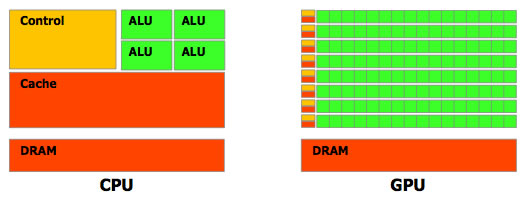
\includegraphics[width=.80\textwidth]{comparacao_GPU_CPU.png}
  \caption{Imagem comparando de forma simplifica a arquitetura dos processadores. Do lado esquerdo a arquitetura de uma Unidade de Processamento Central, muito espaço para o cache e a unidade de comtrole. Do lado direto uma unidade de processamento Gráfica, como uma grande região segmentada dedicada a computação aritimética e lógica}
  \label{fig:cpuvsgpu}
\end{figure}

\section{História das GPU e GPGPU}

  Na Figura~\ref{fig:cpuvsgpu} texto texto

  era uma vez...

\section{Bibliotecas: OpenCL e CUDA}
  o que são e como funcionam
  porque escolhemos cuda?
